\documentclass[11pt]{amsart}
\usepackage[margin=1in]{geometry}
\usepackage{amsmath,amssymb,amsthm,mathtools}
\usepackage[hidelinks]{hyperref}
\usepackage{setspace}
\setstretch{1.14}
\usepackage{tikz}
\usetikzlibrary{positioning,arrows.meta}

\title[Octonionic Action and Uniqueness]{Octonionic Action from the HQIV-LEAN Variational Layer:\\
Derivation, Holonomy Alignment, and a Tiered Uniqueness Thesis}
\author{Steven Ettinger Jr}
\address{Independent Researcher}
\email{steven@disregardfiat.tech}
\date{Preprint v3 --- \today}

\newtheorem{theorem}{Theorem}[section]
\newtheorem{lemma}[theorem]{Lemma}
\newtheorem{proposition}[theorem]{Proposition}
\newtheorem{definition}[theorem]{Definition}
\newtheorem{remark}[theorem]{Remark}
\newtheorem{example}[theorem]{Example}

\begin{document}

\begin{abstract}
This manuscript is a variational sequel to \cite{hqiv-so8-paper} and \cite{hqiv-3d-growth-paper}. Those works package discrete null-shell growth, a normalized cumulative phase readout \(\mathcal{R}\), an explicit phase-lift generator \(\Delta\), and machine-checked Lie closure \(G_2\cup\{\Delta\}\Rightarrow\mathfrak{so}(8)\) on the HQVM octonionic seed. Here we center the \emph{action} layer already present in the HQIV-LEAN library: a discrete octonion-indexed gauge potential \(A^a{}_\mu\), field strength \(F^a{}_{\mu\nu}\), O--Maxwell Lagrangian, Euler--Lagrange covector, gravitational constraint action tied to the HQVM Friedmann identity, and the holonomy glue that re-packages the \emph{same} \(F\) data as abelian plaquette transports with a proved cyclic Stokes identity. The holonomy bridge matters because it ties the variational kinetic aggregate to Wilson-type defects on the minimal \(\mathrm{Fin}\,4\) cycle without changing the underlying discrete flux---the same bookkeeping the rapidity layer uses before Lie closure.

We state with file-level precision which claims are \emph{proved in Lean} (Euler--Lagrange identities matching the discrete divergence of \(F\), cyclic flux sum zero, two-sided bounds comparing \(L_O\) kinetic to cyclic Wilson squares, Friedmann constraint as \(S_{\mathrm{grav}}=0\)) and which steps remain narrative or scaffolded (translation maps to continuum notation, manifold integration wrappers, path-integral measure choices). The \emph{tiered uniqueness thesis} is the paper's conceptual payoff: (I)~within the declared polynomial gauge ansatz, the EL slot is rigid---the discrete implementation is the exact finite-difference analogue of the continuum Maxwell pattern; (II)~Hurwitz rigidity and eight-dimensional division-algebra uniqueness align the \(\mathrm{Fin}\,8\) carrier with triality/\(\mathrm{Spin}(8)\) and the certified \(G_2\cup\{\Delta\}\) seed; (III)~a structured Tier~III \emph{translation} program (continuum convenience rewriting, paired Einstein/\(G_2\) stationarity packaging, associator/measure interfaces) replaces a single vague conjecture. The observable universe is the whole universe in the HQIV ontology, so no continuum limit is required or desired for foundational validity; continuum formulas are used only as convenience coordinates for comparison with standard literature. The goal is to advance the action story on its own audit spine without folding it into the shell-combinatorics graph of the predecessors. For readers coming from lattice gauge theory, the holonomy lemmas position the same \(F\) slots where Wilson plaquette language applies \cite{wilson1974,creutz1983}. We also name \emph{lapse dragging}: the HQVM identification of the cumulative lapse increment \(\phi t/c\) above the Newtonian \(\Phi\) piece with the \emph{same} auxiliary scalar that enters \(\mathcal{L}_\phi\) and \(G_{\mathrm{eff}}(\phi)=\phi^{3/5}\) (\path{HQVM_lapse}, \path{same_phi_in_O_Maxwell_and_HQVM} in \path{GRFromMaxwell.lean}); Remark~\ref{rem:lapse-lambda} records sample \(G_{\mathrm{eff}}/G_0\) ratios and links that single-\(\alpha\) pipeline to galactic rotation-curve phenomenology in the Jacobson/Brodie horizon picture \cite{jacobson1995,brodie2026}.
\end{abstract}
\maketitle

% Shared reader contract: patch QFT + discrete numerics.
% From papers/*.tex:     % Shared reader contract: patch QFT + discrete numerics.
% From papers/*.tex:     % Shared reader contract: patch QFT + discrete numerics.
% From papers/*.tex:     \input{include/patch_theory_messaging.tex}
% From papers/paper/*.tex: \input{../include/patch_theory_messaging.tex}

\paragraph{Patch QFT and discrete numerics (reader contract).}
HQIV is formulated as a \emph{patch theory}: quantum fields, actions, and physical readouts are attached to discrete patches---shell indices $m\in\mathbb{N}$, finite spacetime index types (e.g.\ $\mathrm{Fin}\,4$), and horizon-limited charts---rather than to a hypothetical fundamental smooth spacetime obtained as a mesh-refinement or ultraviolet limit.
Accordingly, when this text refers to ``QFT,'' it means \emph{patch QFT}: patching rules, finite measurement ledgers, and variational identities on the discrete spine; it is not the claim that the theory is \emph{defined} by recovering ordinary continuum quantum field theory through such a limit.
The numbers that admit the sharpest statements---mass and coupling ladders, curvature ratios, shell thermodynamics, and rational witnesses in \texttt{HQIV\_LEAN}---are objects of \emph{discrete mathematics} on $\mathbb{N}$ (combinatorial growth, cumulative simplex ledgers) together with the ordered field $\mathbb{R}$ as used in the proof assistant for analysis, bounds, and phenomenological display.
Smooth-manifold or continuum field notation, when it appears, is a \emph{translation layer} for comparison with standard physics literature; it does not supersede the discrete definitions.

% From papers/paper/*.tex: % Shared reader contract: patch QFT + discrete numerics.
% From papers/*.tex:     \input{include/patch_theory_messaging.tex}
% From papers/paper/*.tex: \input{../include/patch_theory_messaging.tex}

\paragraph{Patch QFT and discrete numerics (reader contract).}
HQIV is formulated as a \emph{patch theory}: quantum fields, actions, and physical readouts are attached to discrete patches---shell indices $m\in\mathbb{N}$, finite spacetime index types (e.g.\ $\mathrm{Fin}\,4$), and horizon-limited charts---rather than to a hypothetical fundamental smooth spacetime obtained as a mesh-refinement or ultraviolet limit.
Accordingly, when this text refers to ``QFT,'' it means \emph{patch QFT}: patching rules, finite measurement ledgers, and variational identities on the discrete spine; it is not the claim that the theory is \emph{defined} by recovering ordinary continuum quantum field theory through such a limit.
The numbers that admit the sharpest statements---mass and coupling ladders, curvature ratios, shell thermodynamics, and rational witnesses in \texttt{HQIV\_LEAN}---are objects of \emph{discrete mathematics} on $\mathbb{N}$ (combinatorial growth, cumulative simplex ledgers) together with the ordered field $\mathbb{R}$ as used in the proof assistant for analysis, bounds, and phenomenological display.
Smooth-manifold or continuum field notation, when it appears, is a \emph{translation layer} for comparison with standard physics literature; it does not supersede the discrete definitions.


\paragraph{Patch QFT and discrete numerics (reader contract).}
HQIV is formulated as a \emph{patch theory}: quantum fields, actions, and physical readouts are attached to discrete patches---shell indices $m\in\mathbb{N}$, finite spacetime index types (e.g.\ $\mathrm{Fin}\,4$), and horizon-limited charts---rather than to a hypothetical fundamental smooth spacetime obtained as a mesh-refinement or ultraviolet limit.
Accordingly, when this text refers to ``QFT,'' it means \emph{patch QFT}: patching rules, finite measurement ledgers, and variational identities on the discrete spine; it is not the claim that the theory is \emph{defined} by recovering ordinary continuum quantum field theory through such a limit.
The numbers that admit the sharpest statements---mass and coupling ladders, curvature ratios, shell thermodynamics, and rational witnesses in \texttt{HQIV\_LEAN}---are objects of \emph{discrete mathematics} on $\mathbb{N}$ (combinatorial growth, cumulative simplex ledgers) together with the ordered field $\mathbb{R}$ as used in the proof assistant for analysis, bounds, and phenomenological display.
Smooth-manifold or continuum field notation, when it appears, is a \emph{translation layer} for comparison with standard physics literature; it does not supersede the discrete definitions.

% From papers/paper/*.tex: % Shared reader contract: patch QFT + discrete numerics.
% From papers/*.tex:     % Shared reader contract: patch QFT + discrete numerics.
% From papers/*.tex:     \input{include/patch_theory_messaging.tex}
% From papers/paper/*.tex: \input{../include/patch_theory_messaging.tex}

\paragraph{Patch QFT and discrete numerics (reader contract).}
HQIV is formulated as a \emph{patch theory}: quantum fields, actions, and physical readouts are attached to discrete patches---shell indices $m\in\mathbb{N}$, finite spacetime index types (e.g.\ $\mathrm{Fin}\,4$), and horizon-limited charts---rather than to a hypothetical fundamental smooth spacetime obtained as a mesh-refinement or ultraviolet limit.
Accordingly, when this text refers to ``QFT,'' it means \emph{patch QFT}: patching rules, finite measurement ledgers, and variational identities on the discrete spine; it is not the claim that the theory is \emph{defined} by recovering ordinary continuum quantum field theory through such a limit.
The numbers that admit the sharpest statements---mass and coupling ladders, curvature ratios, shell thermodynamics, and rational witnesses in \texttt{HQIV\_LEAN}---are objects of \emph{discrete mathematics} on $\mathbb{N}$ (combinatorial growth, cumulative simplex ledgers) together with the ordered field $\mathbb{R}$ as used in the proof assistant for analysis, bounds, and phenomenological display.
Smooth-manifold or continuum field notation, when it appears, is a \emph{translation layer} for comparison with standard physics literature; it does not supersede the discrete definitions.

% From papers/paper/*.tex: % Shared reader contract: patch QFT + discrete numerics.
% From papers/*.tex:     \input{include/patch_theory_messaging.tex}
% From papers/paper/*.tex: \input{../include/patch_theory_messaging.tex}

\paragraph{Patch QFT and discrete numerics (reader contract).}
HQIV is formulated as a \emph{patch theory}: quantum fields, actions, and physical readouts are attached to discrete patches---shell indices $m\in\mathbb{N}$, finite spacetime index types (e.g.\ $\mathrm{Fin}\,4$), and horizon-limited charts---rather than to a hypothetical fundamental smooth spacetime obtained as a mesh-refinement or ultraviolet limit.
Accordingly, when this text refers to ``QFT,'' it means \emph{patch QFT}: patching rules, finite measurement ledgers, and variational identities on the discrete spine; it is not the claim that the theory is \emph{defined} by recovering ordinary continuum quantum field theory through such a limit.
The numbers that admit the sharpest statements---mass and coupling ladders, curvature ratios, shell thermodynamics, and rational witnesses in \texttt{HQIV\_LEAN}---are objects of \emph{discrete mathematics} on $\mathbb{N}$ (combinatorial growth, cumulative simplex ledgers) together with the ordered field $\mathbb{R}$ as used in the proof assistant for analysis, bounds, and phenomenological display.
Smooth-manifold or continuum field notation, when it appears, is a \emph{translation layer} for comparison with standard physics literature; it does not supersede the discrete definitions.


\paragraph{Patch QFT and discrete numerics (reader contract).}
HQIV is formulated as a \emph{patch theory}: quantum fields, actions, and physical readouts are attached to discrete patches---shell indices $m\in\mathbb{N}$, finite spacetime index types (e.g.\ $\mathrm{Fin}\,4$), and horizon-limited charts---rather than to a hypothetical fundamental smooth spacetime obtained as a mesh-refinement or ultraviolet limit.
Accordingly, when this text refers to ``QFT,'' it means \emph{patch QFT}: patching rules, finite measurement ledgers, and variational identities on the discrete spine; it is not the claim that the theory is \emph{defined} by recovering ordinary continuum quantum field theory through such a limit.
The numbers that admit the sharpest statements---mass and coupling ladders, curvature ratios, shell thermodynamics, and rational witnesses in \texttt{HQIV\_LEAN}---are objects of \emph{discrete mathematics} on $\mathbb{N}$ (combinatorial growth, cumulative simplex ledgers) together with the ordered field $\mathbb{R}$ as used in the proof assistant for analysis, bounds, and phenomenological display.
Smooth-manifold or continuum field notation, when it appears, is a \emph{translation layer} for comparison with standard physics literature; it does not supersede the discrete definitions.


\paragraph{Patch QFT and discrete numerics (reader contract).}
HQIV is formulated as a \emph{patch theory}: quantum fields, actions, and physical readouts are attached to discrete patches---shell indices $m\in\mathbb{N}$, finite spacetime index types (e.g.\ $\mathrm{Fin}\,4$), and horizon-limited charts---rather than to a hypothetical fundamental smooth spacetime obtained as a mesh-refinement or ultraviolet limit.
Accordingly, when this text refers to ``QFT,'' it means \emph{patch QFT}: patching rules, finite measurement ledgers, and variational identities on the discrete spine; it is not the claim that the theory is \emph{defined} by recovering ordinary continuum quantum field theory through such a limit.
The numbers that admit the sharpest statements---mass and coupling ladders, curvature ratios, shell thermodynamics, and rational witnesses in \texttt{HQIV\_LEAN}---are objects of \emph{discrete mathematics} on $\mathbb{N}$ (combinatorial growth, cumulative simplex ledgers) together with the ordered field $\mathbb{R}$ as used in the proof assistant for analysis, bounds, and phenomenological display.
Smooth-manifold or continuum field notation, when it appears, is a \emph{translation layer} for comparison with standard physics literature; it does not supersede the discrete definitions.


\section{Logical placement and reader contract}
\label{sec:placement}

\subsection{Predecessors}

\cite{hqiv-so8-paper} gives the chain
\[
\text{uniform growth} \Longrightarrow K \Longrightarrow \Omega \Longrightarrow \mathcal{R}
\Longrightarrow \Delta \Longrightarrow \langle G_2,\Delta\rangle_{\mathrm{Lie}}=\mathfrak{so}(8)
\]
under explicit imports (quadratic shell law, \(\alpha=3/5\) normalization story, Fano octonion model, \((e_1,e_7)\) plane). \cite{hqiv-3d-growth-paper} isolates the quadratic-versus-cubic dimensional hinge in \(3{+}1\), records conditional forcing theorems in \path{Hqiv/Story/CausalRapidityForcing.lean}, and develops Hurwitz/triality narrative with careful scope.

\subsection{Where this paper sits in the three-layer stack}

It is useful to picture HQIV formalization as three layers that \emph{compose} in the repository narrative but have different logical strengths. The \textbf{discrete growth layer} (shell counts, \(K,\Omega,\mathcal{R}\), lattice--\(\alpha\) coherence) is the strongest combinatorial spine; the \textbf{Lie closure layer} (\(G_2\cup\{\Delta\}\Rightarrow\mathfrak{so}(8)\) on explicit matrices) is a certified linear-algebra certificate once seeds are fixed; the \textbf{variational layer} of the present manuscript (\path{Hqiv/Physics/Action.lean} and holonomy glue) packages equations of motion and constraints as stationarity of explicit functionals over the same octonion-indexed cutoff. This paper does \emph{not} merge those layers into a single implication from poset axioms; it documents the third layer precisely and explains how it is designed to interoperate with the first two through shared parameters \((\alpha,\phi)\).

\subsection{What this paper adds (Lean modules)}
\label{subsec:adds}

\begin{itemize}
\item \textbf{Discrete O--Maxwell action and EL identities} (\path{Hqiv/Physics/Action.lean}; Sect.~\ref{sec:discrete}). Definitions \path{F_from_A}, \path{L_O_kinetic}, \path{L_O_Maxwell_general}, \path{EL_O_general}, theorems \path{action_O_Maxwell_EL_eq_emergent_general}, superposition \path{action_O_Maxwell_general_add_J}.
\item \textbf{Gravity constraint and total action} (\path{Hqiv/Physics/Action.lean}; Sect.~\ref{sec:grav}). \path{S_HQVM_grav}, \path{S_HQVM_grav_zero_iff_Friedmann}, \path{action_total_general}, \path{action_total_general_add_J}, \path{equations_from_action}.
\item \textbf{Holonomy alignment on the same \(F\) slots} (\path{Hqiv/Physics/ActionHolonomyGlue.lean}; Sect.~\ref{sec:holonomy}). \path{sum_F_cyclicIndex_eq_zero}, \path{discreteSquareHolonomy_F_cyclic_eq_one}, \path{L_O_kinetic_le_neg_quarter_sum_cyclic_wilson_sq}, \path{L_O_kinetic_ge_neg_half_sum_cyclic_wilson_sq}, \path{L_O_kinetic_two_sided_cyclic_wilson_sq}.
\item \textbf{Weak/Higgs Tier-III scaffold on top of the proved abelian core} (\path{Hqiv/Physics/WeakHiggsFromOMaxwellScaffold.lean}; Sect.~\ref{sec:weak-higgs-scaffold}). Definitions \path{weakF}, \path{L_weak_kinetic}, \path{higgsPotential}, \path{lockinVev}, and reduction/status theorems \path{weakF_reduces_to_abelian}, \path{lockinVev_sq_eq_eta_paper}, \path{action_O_weak_higgs_reduces_exactly_to_action_O_Maxwell}, \path{weakHiggs_triality_tilt_average_eq_one}.
\end{itemize}

\subsection{Scope and not claimed}
\label{subsec:not-claimed}

\begin{itemize}
\item Causal poset axioms \emph{alone} do not imply this action; the quadratic shell law, octonion table, and plane choices remain explicit imports where used.
\item No continuum path integral, anomaly cancellation, or uniqueness of measure is proved here, and none is required for the discrete core claims of this paper.
\item No claim that alternative discrete variational ans\"atze cannot be written off the HQIV design path; Tier~I uniqueness is \emph{internal} to the stated Lagrangian class.
\item The functorial bridge \(\mathcal{R}\rightsquigarrow A\) with analytic error control is deferred to \path{Hqiv/Geometry/ManifoldLagrangianScaffold.lean} and \path{LatticeContinuumActionCoincidence} (Sect.~\ref{sec:bridge}).
\end{itemize}

\section{Discrete O--Maxwell action}
\label{sec:discrete}

Fix octonion channel index \(a\in \mathrm{Fin}\,8\) and spacetime index \(\mu,\nu\in \mathrm{Fin}\,4\) as in the library.

\begin{definition}[Discrete field strength (Lean: \path{F_from_A})]
\label{def:F}
For \(A : \mathrm{Fin}\,8 \to \mathrm{Fin}\,4 \to \mathbb{R}\),
\[
F^a{}_{\mu\nu}(A) := A^a{}_\nu - A^a{}_\mu .
\]
\end{definition}

\begin{definition}[Kinetic and source densities (Lean)]
\label{def:kinetic-source}
The kinetic aggregate is (\path{L_O_kinetic})
\begin{equation}
\label{eq:Lkin-expanded}
\mathcal{L}_{\mathrm{kin}}(A)
:= -\frac14 \sum_{a\in \mathrm{Fin}\,8}\;\sum_{\mu,\nu\in \mathrm{Fin}\,4}
\frac{\bigl(F^a{}_{\mu\nu}(A)\bigr)^2}{2}.
\end{equation}
The factor \(\tfrac12\) inside the sum implements antisymmetric bookkeeping while summing over all ordered pairs \((\mu,\nu)\). The source interaction for \(J_{\mathrm{src}} : \mathrm{Fin}\,8 \to \mathrm{Fin}\,4 \to \mathbb{R}\) is (\path{L_O_source_general})
\begin{equation}
\label{eq:Lsource-expanded}
\mathcal{L}_{\mathrm{src}}(J_{\mathrm{src}},A)
:= \sum_{a\in \mathrm{Fin}\,8}\;\sum_{\nu\in \mathrm{Fin}\,4} (J_{\mathrm{src}})^a{}_\nu\, A^a{}_\nu .
\end{equation}
\end{definition}

\begin{definition}[Full O--Maxwell density and action cell (Lean)]
\label{def:LOmaxwell}
For \(\phi_{\mathrm{val}}>-1\), the \(\phi\)-coupling term is (\path{L_O_phi_coupling})
\[
\mathcal{L}_\phi(A,\phi_{\mathrm{val}})
:= \alpha\,\log(\phi_{\mathrm{val}}+1)\sum_{\nu\in \mathrm{Fin}\,4} (\mathrm{grad}_\phi)_\nu\, A^0{}_\nu ,
\]
with \((\mathrm{grad}_\phi)_\nu = \)\path{grad_phi} \(\nu\) (currently the zero placeholder in \path{Action.lean}; continuum gradients use \path{ContinuumOmaxwellClosure}). The full density is
\[
\mathcal{L}_O[J_{\mathrm{src}}](A,\phi_{\mathrm{val}})
:= \mathcal{L}_{\mathrm{kin}}(A) + 4\pi\,\mathcal{L}_{\mathrm{src}}(J_{\mathrm{src}},A) + \mathcal{L}_\phi(A,\phi_{\mathrm{val}}),
\]
(\path{L_O_Maxwell_general}). The \emph{action cell} is the same real number (\path{action_O_Maxwell_general}).
\end{definition}

\begin{theorem}[Discrete Euler--Lagrange matches divergence of \(F\) minus sources (Lean)]
\label{thm:EL}
For \path{J_src}, \(A\), \(\phi_{\mathrm{val}}\) with \(\phi_{\mathrm{val}}+1>0\), the component \path{EL_O_general} at \((a,\nu)\) equals
\[
\sum_{\mu\in \mathrm{Fin}\,4} F^a{}_{\mu\nu}(A) - 4\pi (J_{\mathrm{src}})^a{}_\nu
-\begin{cases}
\alpha\,\log(\phi_{\mathrm{val}}+1)\,(\mathrm{grad}_\phi)_\nu, & a=0,\\
0, & a\neq 0 .
\end{cases}
\]
This is \path{action_O_Maxwell_EL_eq_emergent_general} (and \path{action_O_Maxwell_EL_eq_emergent} for \path{J_O}).
\end{theorem}

\begin{proof}[Sketch (conceptual; Lean is definitional/rw)]
Vary \(A^b{}_\sigma\to A^b{}_\sigma+\varepsilon\,\delta^b_a\,\delta^\sigma_\nu\) in \(\mathcal{L}_{\mathrm{kin}}\). Each \(F^b{}_{\mu\sigma}\) shifts by \(\varepsilon(\delta^\mu_\sigma-\delta^\mu_\nu)\) when \(\sigma=\nu\), and each \(F^b{}_{\nu\mu}\) shifts by the opposite increment. Collecting coefficients of \(\varepsilon\) produces a telescoping sum over \(\mu\) that yields \(\sum_\mu F^a{}_{\mu\nu}\)---the discrete analogue of \(\partial_\mu F^{\mu\nu}\). The source term \(4\pi J\!\cdot\!A\) contributes \(-4\pi J^a{}_\nu\) to the EL covector, and the \(\phi\)-coupling contributes only on channel \(a=0\) by construction. This is the standard polynomial-gauge calculation carried out on the finite index set.
\end{proof}

\begin{remark}[\(\alpha\), \(\gamma_{\mathrm{HQIV}}\), and the AuxiliaryField ladder]
The imprint \(\alpha=3/5\) enters \(\mathcal{L}_\phi\) explicitly. The same \(\alpha\) is tied to the null-shell curvature density in \path{OctonionicLightCone} (\path{shell_shape}, \path{alpha_eq_3_5}); readers who arrive from the growth manuscript and want the thermodynamic packaging of the imprint fractions (Jacobson/Brodie on horizons, monogamy template) should consult the appendix \emph{Thermodynamic Derivation of the \((\alpha_d,\gamma_d)\) Family} in \cite{hqiv-3d-growth-paper} (Lean anchor \texttt{sec:thermo-derivation} in \path{papers/hqiv_3d_causal_growth_octonionic_gauge.tex}). The auxiliary scalar follows the temperature ladder in \path{Hqiv/Geometry/AuxiliaryField.lean}: \path{phi_of_shell} at shell index \texttt{m} equals \path{phiTemperatureCoeff} divided by \path{T}\texttt{(m)}, with \path{phiTemperatureCoeff} the proved constant \texttt{2} (\path{phiTemperatureCoeff_eq_two}), and \path{shell_shape_in_terms_of_phi} rewrites the shell readout using \(\phi(m)/2=m+1\). On the gravity side, \path{gamma_HQIV} enters the Friedmann coefficient \((3-\gamma_{\mathrm{HQIV}})\) in \path{S_HQVM_grav}; Lean proves \((3-\gamma_{\mathrm{HQIV}})=13/5\) (\path{three_minus_gamma_eq} in \path{Hqiv/Geometry/HQVMetric.lean}). Thus \((\alpha,\gamma)\) is simultaneously the monogamy/unit-split pair from the growth papers and the coupling/normalization pair threading Action, \path{HQVMetric}, and \path{AuxiliaryField}.
\end{remark}

\begin{remark}[Relation to \path{ModifiedMaxwell.emergentMaxwellInhomogeneous_O_general}]
\label{rem:modified-maxwell}
\path{Hqiv/Physics/ModifiedMaxwell.lean} packages the emergent O-sector equation with the same \(-4\pi J_{\mathrm{src}}\) slot and \(\alpha\)-weighted \(\phi\)-gradient correction (via \path{grad_phi} in \path{Action.lean}, the placeholder gradient in \path{ModifiedMaxwell.lean}, and \path{coordsGradientComponents} in \path{ContinuumOmaxwellClosure}). The discrete Action EL uses an explicit \(\sum_\mu F\) surrogate while the emergent file still carries a placeholder \texttt{0.0} for the covariant divergence term; the maintained design contract is \emph{source-slot alignment} between EL and emergent inhomogeneous equations. Completing the identification requires wiring the same \path{coordsGradientComponents} into both sides---already started in \path{ContinuumOmaxwellClosure}.
\end{remark}

\section{Gravitational sector and total action}
\label{sec:grav}

\begin{theorem}[Gravitational constraint equals Friedmann (Lean)]
\label{thm:friedmann}
For \(\phi,\rho_m,\rho_r\in\mathbb{R}\), with \path{S_HQVM_grav} and \path{HQVM_Friedmann_eq} as in the library,
\[
\text{\texttt{S\_HQVM\_grav}}(\phi,\rho_m,\rho_r)=0
\quad\Longleftrightarrow\quad
\text{\texttt{HQVM\_Friedmann\_eq}}\,\phi\,\rho_m\,\rho_r.
\]
This is \path{S_HQVM_grav_zero_iff_Friedmann}. Equivalently, for \(\phi\ge 0\), \path{O_Maxwell_compatible_with_HQVM_GR_homogeneous} rewrites the constraint as \((13/5)\phi^2 = 8\pi\,\phi^{\alpha}(\rho_m+\rho_r)\).
\end{theorem}

\begin{definition}[Total action and current superposition (Lean)]
\label{def:total}
Write \(\mathcal{S}_O[J_{\mathrm{src}}](A,\phi_{\mathrm{val}}):=\mathcal{L}_O[J_{\mathrm{src}}](A,\phi_{\mathrm{val}})\) for the O--Maxwell cell and let \(\mathcal{S}_{\mathrm{grav}}(\phi,\rho_m,\rho_r)\) denote \path{S_HQVM_grav} evaluated at \((\phi,\rho_m,\rho_r)\). The total cell is
\[
\mathcal{S}_{\mathrm{tot}}[J_{\mathrm{src}}](A,\phi,\rho_m,\rho_r)
:= \mathcal{S}_O[J_{\mathrm{src}}](A,\phi) + \mathcal{S}_{\mathrm{grav}}(\phi,\rho_m,\rho_r),
\]
as defined by \path{action_total_general}.
For two sources, Lean proves
\begin{multline}
\label{eq:superposition-correction}
\mathcal{S}_{\mathrm{tot}}[J_1+J_2](A,\phi,\rho_m,\rho_r)
= \mathcal{S}_{\mathrm{tot}}[J_1](A,\phi,\rho_m,\rho_r)
+ \mathcal{S}_{\mathrm{tot}}[J_2](A,\phi,\rho_m,\rho_r) \\
{}- \mathcal{L}_{\mathrm{kin}}(A) - \mathcal{L}_\phi(A,\phi) - \mathcal{S}_{\mathrm{grav}}(\phi,\rho_m,\rho_r).
\end{multline}
This is \path{action_total_general_add_J} (built from \path{action_O_Maxwell_general_add_J}). The O--Maxwell part alone satisfies the simpler linearity in \(J\) only for the \(4\pi\,J\!\cdot\!A\) piece; the kinetic and \(\phi\) terms are shared, so naive addition of two full densities double-counts those shared blocks.
\end{definition}

\begin{example}[Flat potential, trivial current, balanced densities]
\label{ex:simultaneous}
Take \(A^a{}_\mu\equiv 0\) so \(F^a{}_{\mu\nu}=0\) and \(\mathcal{L}_{\mathrm{kin}}=0\); take \path{J_O}\(\equiv 0\) so \(\mathcal{L}_{\mathrm{src}}=0\); take \path{grad_phi}\(\equiv 0\) so \(\mathcal{L}_\phi=0\). Then \(\mathcal{S}_O=0\). Choose \(\phi=1\) (Hubble reference in natural units). Friedmann requires \((13/5)\phi^2 = 8\pi\,\phi^{\alpha}(\rho_m+\rho_r)\) with \(\alpha=3/5\), hence \(\rho_m+\rho_r = 13/(40\pi)\). For these values \(\mathcal{S}_{\mathrm{grav}}=0\) and \path{EL_O} reduces to \(\sum_\mu F=0\), which holds trivially. This is the same decoupled ``zero sector'' used in \path{equations_from_action} for illustration: gravity is a constraint on \((\phi,\rho)\); gauge EL is a separate stationarity problem in \(A\) once \(J\) and \(\phi\) data are fixed.
\end{example}

\begin{remark}[\texorpdfstring{Lapse dragging, lapse-corrected GR, and the demystified $\Lambda$}{Lapse dragging, lapse-corrected GR, and demystified Lambda}]
\label{rem:lapse-lambda}
The constraint \(\mathcal{S}_{\mathrm{grav}}=0\) of Theorem~\ref{thm:friedmann} is \emph{not} the textbook flat FLRW equation of Einstein GR with a fundamental cosmological constant \(\Lambda\),
\[
H^2=\frac{8\pi G}{3}\,\rho_{\mathrm{tot}}+\frac{\Lambda c^2}{3}.
\]
Instead, for \(\phi\ge 0\), Lean rewrites the HQVM Friedmann identity as (\path{O_Maxwell_compatible_with_HQVM_GR_homogeneous})
\begin{equation}
\label{eq:hqvm-friedmann-explicit}
\frac{13}{5}\,\phi^2 = 8\pi\,G_{\mathrm{eff}}(\phi)\,(\rho_m+\rho_r),
\qquad G_{\mathrm{eff}}(\phi)=\phi^{\alpha},\quad \alpha=\frac35
\end{equation}
(\path{G_eff_eq}), where \((3-\gamma_{\mathrm{HQIV}})=13/5\) is the unit-split/monogamy coefficient (\path{three_minus_gamma_eq}). There is therefore \textbf{no independent \(\Lambda\) knob}: whatever plays the role of a ``dark'' constant term in a standard frame is packaged here into the \(\phi\)-dependent coupling \(G_{\mathrm{eff}}\) and the fixed rational prefactor inherited from the same \((\alpha,\gamma)\) ledger that the thermodynamic appendix of \cite{hqiv-3d-growth-paper} derives from Jacobson/Brodie horizon bookkeeping. In the HQVM narrative, \(\phi\) is the relative-observer energy normalizer (auxiliary field / temperature ladder), not an ad hoc fifth force; identifying \(H\) with \(\phi\) in the homogeneous sector is the calibration already used in \path{GRFromMaxwell.lean}. The seed map \(\mathcal{R}\rightsquigarrow A\) of Subsection~\ref{subsec:minimal-seed} makes the coupling explicit at the variational level: the same readout increments and \(\log(\phi+1)\) weighting that thread into \(\mathcal{L}_\phi\) also enter the gravitational constraint through \(\phi\) and \(\alpha\). A Tier~III continuum limit would target Einstein-type dynamics with an \emph{emergent}, normalization-sensitive effective vacuum contribution---not a fitted fundamental \(\Lambda\).

\medskip
\noindent\textbf{Lapse dragging.}
In synchronous-comoving gauge the HQVM lapse is \(N=1+\Phi+\phi t/c\) (\path{HQVM_lapse} in \path{HQVMetric.lean}). Following \cite{jacobson1995,brodie2026}, we use the term \emph{lapse dragging} for the coupling of the cumulative horizon phase \(\phi t/c\) to proper time \emph{and} to the same \(\phi\) slot that appears in \(\mathcal{L}_\phi\) and in~\eqref{eq:hqvm-friedmann-explicit}. Lean packages the identification of that slot across the O--Maxwell and homogeneous GR branches as \path{same_phi_in_O_Maxwell_and_HQVM}; the imprint exponent is the same statement as \path{same_alpha_in_O_Maxwell_and_HQVM}. Thus ``lapse dragging'' is not an extra postulate: it is the visible name for the shared \(\phi\) morphism already audited in \path{GRFromMaxwell.lean}.

\begin{table}[ht]
\centering
\small
\caption{Effective gravitational coupling in natural units (\(G_0=1\), \texttt{G0\_eq}): \(G_{\mathrm{eff}}(\phi)/G_0=\phi^{3/5}\) from \texttt{G\_eff\_eq} (rounded).}
\label{tab:Geff-numerics}
\begin{tabular}{@{}c@{\quad}c@{}}
\hline
\(\phi\) & \(G_{\mathrm{eff}}(\phi)/G_0=\phi^{3/5}\) \\
\hline
\(0.5\) & \(0.660\) \\
\(0.8\) & \(0.875\) \\
\(1.0\) & \(1.000\) \\
\(1.2\) & \(1.116\) \\
\(1.5\) & \(1.275\) \\
\(2.0\) & \(1.516\) \\
\hline
\end{tabular}
\end{table}

\medskip
\noindent\textbf{Galactic rotation curves.}
Flat disk kinematics in the low-acceleration regime are standard targets for modified inertia derived from horizon overlap \cite{brodie2026}. The \emph{same} \(\alpha=3/5\) that enters \(G_{\mathrm{eff}}(\phi)=\phi^{\alpha}\) and \(\mathcal{L}_\phi\) is the imprint forced by the discrete light-cone layer (\path{alpha_eq_3_5}); phenomenologically, a running \(G_{\mathrm{eff}}\) tied to \(\phi\) and a Brodie-type inertia factor \(f(a_{\mathrm{loc}},\phi)\) are two faces of one horizon bookkeeping constraint at different kinematic scales. Table~\ref{tab:Geff-numerics} makes the cosmological side of that bookkeeping numerically concrete; linking disk \(v(r)\) data to the same audited \(\alpha\) is then a Tier~III continuum/stationarity task (paired Einstein and matter action stationarity in Sect.~\ref{sec:outlook}), not a new parameter at Tier~I.
\end{remark}

\begin{remark}[Superposition discipline (\texorpdfstring{\texttt{action\_total\_general\_add\_J}}{action_total_general_add_J})]
\label{rem:superposition}
Physically, adding two current systems \(J_1+J_2\) should increase only the interaction energy \(\int J\!\cdot\!A\) (here, the discrete \(4\pi\,J\!\cdot\!A\) term) while retaining a \emph{single} copy of the gauge-field self-energy and a \emph{single} Friedmann constraint for the shared \((\phi,\rho)\). Equation~\eqref{eq:superposition-correction} is the bookkeeping correction that enforces ``no double counting'' of \(\mathcal{L}_{\mathrm{kin}}\), \(\mathcal{L}_\phi\), and \(\mathcal{S}_{\mathrm{grav}}\) when concatenating two source packages into one variational cell. This matches the broader HQIV audit discipline: only book-kept morphisms count as physical intermediates.
\end{remark}

\begin{remark}[\texorpdfstring{\texttt{equations\_from\_action}}{equations_from_action}]
The packaged theorem \path{equations_from_action} records the joint pattern: Friedmann arises as the gravitational constraint, while the gauge sector's EL identities are the discrete equations of motion at the chosen potential.
\end{remark}

\section{Holonomy alignment and the same \texorpdfstring{$F$}{F} data}
\label{sec:holonomy}

\subsection{Cyclic Stokes and trivial plaquette holonomy}

\begin{lemma}[Cyclic flux sum (\texorpdfstring{\texttt{sum\_F\_cyclicIndex\_eq\_zero}}{sum_F_cyclicIndex_eq_zero})]
\label{lem:stokes}
For every channel \(a\) and every potential \(A\),
\[
\sum_{i\in \mathrm{Fin}\,4} F^a{}_{i,\,i+1}(A) = 0 .
\]
\end{lemma}

\paragraph{Expository telescoping (\texorpdfstring{\texttt{sum\_F\_cyclicIndex\_eq\_zero}}{sum_F_cyclicIndex_eq_zero}).}
Unfold \(F^a{}_{i,i+1}=A^a{}_{i+1}-A^a{}_i\) for \(i=0,1,2,3\) on the cyclic \(\mathrm{Fin}\,4\) line, with \(3+1=0\) in the index ring. The sum is
\[
(A^a_1{-}A^a_0)+(A^a_2{-}A^a_1)+(A^a_3{-}A^a_2)+(A^a_0{-}A^a_3)=0,
\]
purely by cancellation; no input from octonion multiplication is used---only the abelian group structure of \(\mathbb{R}\) under addition. This is the discrete face of Stokes' theorem on the minimal spacetime cycle at the cutoff.

\begin{lemma}[Trivial abelian holonomy on the cycle (\texorpdfstring{\texttt{discreteSquareHolonomy\_F\_cyclic\_eq\_one}}{discreteSquareHolonomy})]
\label{lem:hol-one}
With transports \path{linearEnd} \((\delta)(x)=x+\delta\), the cyclic plaquette holonomy built from edges \(F^a{}_{i,i+1}\) equals the identity: \path{discreteSquareHolonomy_F_cyclic_eq_one}.
\end{lemma}

\begin{lemma}[Kinetic vs.\ cyclic Wilson squares (\texorpdfstring{\texttt{L\_O\_kinetic\_two\_sided\_cyclic\_wilson\_sq}}{L_O_kinetic_two_sided})]
\label{lem:wilson-bounds}
For any \(x\in\mathbb{R}\), \path{L_O_kinetic_two_sided_cyclic_wilson_sq} gives
\[
-\frac12 \sum_{a,i} \bigl((U^a_i x-x)^2\bigr)
\;\le\; \mathcal{L}_{\mathrm{kin}}(A)
\;\le\; -\frac14 \sum_{a,i} \bigl((U^a_i x-x)^2\bigr),
\]
where each \(U^a_i\) is translation on \(\mathbb{R}\) by the edge flux \(F^a{}_{i,i+1}\) (\path{linearEnd} in \path{ActionHolonomyGlue.lean}). Thus the global variational kinetic is bounded above and below by sums of squared abelian Wilson defects on the cyclic edges.
\end{lemma}

\begin{table}[ht]
\caption{Variational vs.\ holonomy reading of the same \(F\) slots (\texorpdfstring{\texttt{Hqiv/Physics/ActionHolonomyGlue.lean}}{ActionHolonomyGlue}).}
\label{tab:two-views}
\centering
\small
\begin{tabular}{@{}p{2.6cm}p{3.4cm}p{3.4cm}p{3.6cm}@{}}
\hline
Quantity & Variational meaning & Holonomy meaning & Lean identifier \\
\hline
\(F^a{}_{\mu\nu}\) & Kinetic density \(-\tfrac14 F^2\) summed over all \((\mu,\nu)\) & Edge flux for abelian transport & \path{F_from_A} \\
\(\sum_i F^a{}_{i,i+1}\) & Implied constraint on cyclic subset of pairs & Discrete Stokes: vanishing sum around cycle & \path{sum_F_cyclicIndex_eq_zero} \\
\(\prod_i U^a_i\) & (not used directly in \(L\)) & Identity holonomy on closed plaquette & \path{discreteSquareHolonomy_F_cyclic_eq_one} \\
\(\mathcal{L}_{\mathrm{kin}}\) & Global \(8\times 4\times 4\) aggregate & Bounded by cyclic Wilson squares & \path{L_O_kinetic_le_neg_quarter_sum_cyclic_wilson_sq}, \path{L_O_kinetic_ge_neg_half_sum_cyclic_wilson_sq} \\
\hline
\end{tabular}
\end{table}

\begin{remark}[\texorpdfstring{$\mathrm{SO}(8)$ action as internal wave-function transport}{SO8 wave-function transport}]
\label{rem:so8-wavefunction}
The \(\mathfrak{so}(8)\) generators that realize the certified \(G_2\cup\{\Delta\}\) closure act on the octonion-indexed components of the gauge potential \(A^a{}_\mu\) (\(a\in \mathrm{Fin}\,8\)) precisely as infinitesimal rotations of an \(8\)-component internal ``wave function.'' Left-multiplication by the imaginary units supplies the skew-adjoint operators \(L(e_i)\in\mathfrak{so}(8)\) that rotate one octonion direction into another while preserving the Euclidean norm on the carrier. The phase-lift generator \(\Delta\) then appears as a distinguished \(\mathrm{U}(1)\)-like rotation inside this larger structure, consistent with the normalized cumulative phase readout \(\mathcal{R}\) of \cite{hqiv-so8-paper}. In this reading the abelian plaquette transports of Lemma~\ref{lem:hol-one} are literally parallel-transport operators for the internal wave function along the minimal \(\mathrm{Fin}\,4\) cycle. The interpretation is motivational and does not modify any Lean-proved statement; it simply renders manifest why the eight-dimensional normed division algebra is the natural carrier once phase information and curvature are already present in the HQIV pipeline.
\end{remark}

\paragraph{Physical interpretation.}
The HQIV null-shell law is quadratic in the shell index while coarse spatial ball counting is cubic \cite{hqiv-3d-growth-paper}; the curvature channel built on that law feeds \(\alpha\) and hence both monogamy bookkeeping and the variational \(\phi\)-coupling (Remark in Sect.~\ref{sec:discrete}). Table~\ref{tab:two-views} makes the parallel explicit at the \emph{field} level: the same discrete \(F\) enters a global variational kinetic and a local Wilson/Stokes picture, so coercive control on plaquette defects is inherited from the same object that defines the action---the signature that the cutoff is not an arbitrary bookkeeping choice split across modules.

\paragraph{Non-abelian upgrade (pointer).}
Matrix-valued transports inside \path{Function.End} for the same combinatorial cycle are packaged in \path{Hqiv/Physics/DiscretePlaquetteHolonomy.lean}; the glue file stays in the abelian \(\mathbb{R}\) sector to isolate the discrete Stokes identity.

\section{Weak/Higgs extension scaffold (Tier III, typed)}
\label{sec:weak-higgs-scaffold}

To keep the honesty boundary explicit while still advancing formal structure, the repository now includes
\path{Hqiv/Physics/WeakHiggsFromOMaxwellScaffold.lean}. This module is not a replacement for the proved
abelian action layer in \path{Action.lean}; it is a typed extension surface with theorem-level reductions
back to the proved core.

\begin{definition}[Weak-channel and Higgs scaffold objects (Lean)]
The module defines:
\begin{itemize}
\item weak channels \(\texttt{WeakIdx}=\mathrm{Fin}\,3\), weak potentials \(\texttt{WeakPotential}\), and a commutator slot \(\texttt{WeakCommTerm}\);
\item weak field strength
\[
F^{a,\mathrm{weak}}_{\mu\nu}=(W^a_\nu-W^a_\mu)+g_w\,\mathrm{comm}^a_{\mu\nu}
\]
as \path{weakF};
\item weak kinetic density \path{L_weak_kinetic} with the same \(-\tfrac14\sum(\cdot)^2/2\) bookkeeping pattern as \path{L_O_kinetic};
\item octonion-carrier scalar \(\Phi\in\mathbb{R}^8\), norm \path{scalarNormSq}, quartic potential \path{higgsPotential};
\item lock-in vev proxy \(\texttt{lockinVev}:=\sqrt{\eta_{\mathrm{paper}}\Omega_k(m_{\mathrm{lockin}};m_{\mathrm{lockin}})}\).
\end{itemize}
\end{definition}

\begin{theorem}[Immediate reductions to proved channels (Lean)]
\label{thm:weak-higgs-reductions}
The scaffold proves, among others:
\begin{itemize}
\item \path{weakF_reduces_to_abelian} and \path{weakF_diag_eq_zero_of_abelian} for \(g_w=0\), \(\mathrm{comm}=0\);
\item \path{lockinVev_sq_eq_eta_paper} (and \path{lockinVev_eq_sqrt_eta_paper}) under positive lock-in integral, using \path{omega_k_lockin_calibration};
\item \path{action_O_weak_higgs_reduces_to_action_O_Maxwell} and
\path{action_O_weak_higgs_reduces_exactly_to_action_O_Maxwell}, which collapse the extension action to
\path{action_O_Maxwell_general} when weak/Higgs/Yukawa slots are switched off;
\item \path{weakHiggs_triality_tilt_average_eq_one}, importing the already-proved triality CP-tilt averaging identity through the curvature ratio channel.
\end{itemize}
\end{theorem}

\begin{remark}[Status boundary]
This section records a strict separation: the abelian O--Maxwell EL and holonomy statements in Sections~\ref{sec:discrete}--\ref{sec:holonomy} are proved dynamics; the weak/Higgs terms are currently a formally typed Tier-III extension interface with proved reduction laws and consistency links, not yet a completed non-abelian variational closure theorem.
\end{remark}

\section{Design bridge: from growth readout to gauge variables}
\label{sec:bridge}

\subsection{Shared parameters}

\begin{itemize}
\item \textbf{Curvature channel \(\Rightarrow\) \(\alpha\).} The discrete densities \(\rho\), \(K\), \(\Omega\) and the imprint \(\alpha\) are defined in \path{OctonionicLightCone} / \path{HQVMetric}; the same \(\alpha\) appears in \(\mathcal{L}_\phi\) and in \(G_{\mathrm{eff}}(\phi)=\phi^{\alpha}\) (\path{G_eff_eq}).
\item \textbf{Phase readout \(\Rightarrow\) \(\Delta\) and \(\mathfrak{so}(8)\).} \cite{hqiv-so8-paper} constructs \(\Delta\) from the normalized readout; closure spans the \(28\)-dimensional Lie algebra on the HQVM seed.
\item \textbf{Auxiliary \(\phi\).} \path{AuxiliaryField} ties \(\phi(m)\) to the temperature ladder and hence to the same horizon bookkeeping used in the curvature numerator.
\item \textbf{EL \(\Leftrightarrow\) emergent slot.} Stationarity in \(A\) is aligned with the emergent Maxwell source pattern (Remark~\ref{rem:modified-maxwell}).
\end{itemize}

\begin{figure}[ht]
\centering
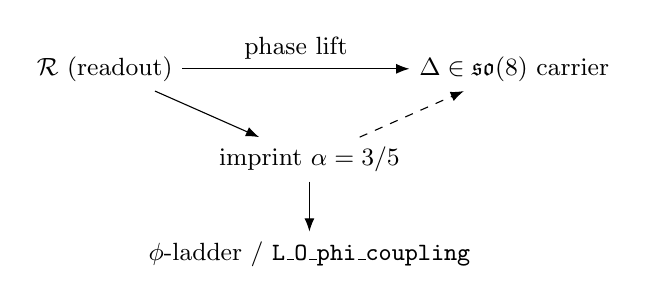
\begin{tikzpicture}[font=\small,>=Latex]
\node (R) at (0,0) {$\mathcal{R}$ (readout)};
\node (D) at (5.2,0) {$\Delta\in\mathfrak{so}(8)$ carrier};
\node (a) at (2.6,-1.15) {imprint \(\alpha=3/5\)};
\node (phi) at (2.6,-2.35) {\(\phi\)-ladder / \texttt{L\_O\_phi\_coupling}};
\draw[->] (R) -- node[above]{phase lift} (D);
\draw[->] (R) -- (a);
\draw[->,dashed] (a) -- (D);
\draw[->] (a) -- (phi);
\end{tikzpicture}
\caption{Design bridge (schematic): the readout pipeline fixes \(\Delta\) in the skew-adjoint octonionic carrier while the curvature imprint \(\alpha\) feeds the auxiliary-field ladder and the action's \(\phi\)-coupling. A fully functorial arrow \(\mathcal{R}\rightsquigarrow A\) is not yet formalized \emph{(see \texttt{ManifoldLagrangianScaffold.lean})}; Subsection~\ref{subsec:minimal-seed} gives an explicit Stokes-compatible seed on the minimal \(\mathrm{Fin}\,4\) cycle.}
\label{fig:bridge}
\end{figure}

\subsection{Functoriality gap}

A morphism \(\mathcal{R}\rightsquigarrow A\) with estimates in a mesh-refinement limit is explicitly deferred to \path{ManifoldLagrangianScaffold.lean} (\path{LagrangianDensity}, chart pullbacks) and the coincidence hypothesis \path{LatticeContinuumActionCoincidence}. Subsection~\ref{subsec:minimal-seed} gives the reference-plaquette seed, now implemented as \path{seedPotentialMinimalCycle} and \path{imprintWeightedReadoutPhase} in \path{Hqiv/Physics/ReadoutGaugeSeed.lean}; functorial extension to larger lattices and error-controlled continuum charts remain Tier~III (Sect.~\ref{sec:outlook}).

\subsection{Minimal seed map \texorpdfstring{$\mathcal{R}\rightsquigarrow A$}{R to A} on the reference \texorpdfstring{$\mathrm{Fin}\,4$}{Fin4} cycle}
\label{subsec:minimal-seed}

This subsection packages a single, fully explicit assignment from the normalized readout and auxiliary ladder to edge fluxes on the smallest nontrivial spacetime cycle, compatible with Lemma~\ref{lem:stokes} and with the abelian holonomy lemmas of Sect.~\ref{sec:holonomy}. The same assignment is now defined and certified in \path{Hqiv/Physics/ReadoutGaugeSeed.lean}. It is the natural first discrete closure of Figure~\ref{fig:bridge} on one plaquette before any continuum limit.

\paragraph{Setup (Lean-identified quantities).}
Fix the calibration shell \path{referenceM} (definitionally tied to the QCD-onset ladder in \path{OctonionicLightCone.lean}; numerically \(4\) in the current repository constants). Under positivity of \path{curvature_integral referenceM}, the partial curvature ratio satisfies \path{omega_k_partial referenceM = 1} (\path{omega_k_partial_at_reference})---the discrete normalization pin for the \(\Omega\) layer in \cite{hqiv-so8-paper}. Write \(\mathcal{R}(n)\) for the normalized cumulative readout (the \(\mathcal{R}\) of \cite{hqiv-so8-paper}, implemented via the \(\Omega\) pipeline) at shell \(n\), and \(\phi(n)\) for \path{phi_of_shell}\(\,n\) from \path{AuxiliaryField}. Define the per-shell readout increment
\[
\delta_{\mathcal{R}}(n):=\mathcal{R}(n+1)-\mathcal{R}(n),
\]
and the imprint-weighted phase increment
\begin{equation}
\label{eq:omega-n}
\omega(n):=\alpha\,\log\bigl(\phi(n)+1\bigr)\,\delta_{\mathcal{R}}(n),
\end{equation}
with \(\alpha=3/5\) as in \path{alpha_eq_3_5}. The phase-lift generator \(\Delta\in\mathfrak{so}(8)\) is fixed in the \((e_1,e_7)\) plane in the HQVM conventions of \cite{hqiv-so8-paper}; let \(\theta\) denote the corresponding polar angle in that plane and set
\[
v^1:=\cos\theta,\qquad v^7:=\sin\theta,\qquad v^a:=0\ \ (a\notin\{1,7\}),
\]
so \(v\in\mathbb{R}^8\) is a unit vector in the \(\Delta\)-direction.

\paragraph{Stokes-compatible flux on the \(\mathrm{Fin}\,4\) cycle.}
For a \emph{fixed} shell label \(n\), assign internal components on directed edges \(i\to i+1\) of the cyclic \(\mathrm{Fin}\,4\) graph by
\begin{equation}
\label{eq:seed-F}
F^1_{i,i+1}(n)=\omega(n)\,s_i\,\cos\theta,\qquad
F^7_{i,i+1}(n)=\omega(n)\,s_i\,\sin\theta,\qquad
F^a_{i,i+1}(n)=0\ \ (a\notin\{1,7\}),
\end{equation}
where \((s_0,s_1,s_2,s_3)=(+1,+1,-1,-1)\). Then \(\sum_{i\in \mathrm{Fin}\,4} F^a_{i,i+1}(n)=0\) for every \(a\) and every \(n\), so Lemma~\ref{lem:stokes} holds \emph{by construction}. Recover potentials on vertices by fixing \(A^a_0(n)=0\) and defining
\[
A^a_{i+1}(n):=A^a_i(n)+F^a_{i,i+1}(n)\qquad (i=0,1,2,3),
\]
with indices interpreted cyclically so that \(A^a_4(n)=A^a_0(n)\); this is the standard pure-gauge freedom on a loop: only the edge data enter \path{F_from_A}, \path{L_O_kinetic}, and the holonomy glue.

\paragraph{Verification (three checks).}
\begin{enumerate}
\item \textbf{Cyclic flux (Lemma~\ref{lem:stokes}).} The choice~\eqref{eq:seed-F} forces \(\sum_i F^a_{i,i+1}(n)=0\) by the alternating signs; equivalently, the vertex potential closes after four steps. No octonion multiplication is used---only \(\mathbb{R}\)-addition, matching the proof style of \path{sum_F_cyclicIndex_eq_zero}.
\item \textbf{Abelian holonomy (Lemma~\ref{lem:hol-one}).} In \path{ActionHolonomyGlue.lean}, cyclic transport is built from \path{linearEnd} applied to the edge variables \(F^a_{i,i+1}\); Lemma~\ref{lem:hol-one} gives the identity holonomy whenever the cyclic sum vanishes. Thus the seed is automatically compatible with the proved \(\mathbb{R}\)-translation picture. An \emph{interpretive} upgrade identifies \(\omega(n)\,v\) with an infinitesimal rotation in the \(\Delta\)-plane inside \(\mathfrak{so}(8)\); the exponential \(\exp(\cdot\,\Delta)\) language belongs to that matrix sector and is not literal \path{linearEnd} composition until a non-abelian transport layer is wired (Sect.~\ref{sec:holonomy}, non-abelian pointer).
\item \textbf{Reference normalization.} At \path{referenceM}, \(\omega(n)\) vanishes whenever \(\delta_{\mathcal{R}}(n)=0\) at that shell (e.g.\ a bookkeeping pivot for the readout increment); then~\eqref{eq:seed-F} collapses to \(F=0\) and, with \(A(\cdot,n)\equiv 0\) at the base vertex, to the flat cycle used in Example~\ref{ex:simultaneous}. More generally, \(\omega(n)\) couples the curvature channel through \(\delta_{\mathcal{R}}\) and the auxiliary factor \(\log(\phi(n)+1)\) that already appears in \(\mathcal{L}_\phi\) (Sect.~\ref{sec:discrete}); the closed form \(\phi(n)=2(n+1)\) from \path{phi_of_shell_closed_form} is independent of the Friedmann \(\phi_{\mathrm{val}}\) normalization in the action cell unless explicitly identified.
\end{enumerate}

\paragraph{Status and scope.}
\path{Hqiv/Physics/ReadoutGaugeSeed.lean} defines \path{seedAProfileAux} (the \(0,\omega c,\omega c,0\) vertex profile equivalent to the alternating edge pattern~\eqref{eq:seed-F}), the gauge potential \path{seedPotentialMinimalCycle}, and the readout-linked scalar \path{imprintWeightedReadoutPhase}. Theorems \path{seedPotentialMinimalCycle_cyclic_sum_F} and \path{seedPotentialMinimalCycle_discrete_holonomy_one} specialize \path{sum_F_cyclicIndex_eq_zero} and \path{discreteSquareHolonomy_F_cyclic_eq_one}; \path{seedPotentialMinimalCycle_of_imprint_increment_zero} encodes flat degeneration when \path{omega_k_partial} has vanishing shell-to-shell increment. What remains outside Lean is promoting shell-indexed potentials \(A(\cdot,n)\) to a global variational field in \path{Action.lean}, proving functoriality and mesh-refinement estimates, and upgrading abelian \path{linearEnd} transport to matrix \(\exp(\cdot\,\Delta)\) data---the Tier~III program in Sect.~\ref{sec:outlook}.

\section{Tiered uniqueness thesis}
\label{sec:tiers}

\subsection{Tier I: EL slot rigidity (formal layer)}

In continuum polynomial abelian gauge theory, \(\mathcal{L}\sim -\tfrac14 F_{\mu\nu}F^{\mu\nu}+J_\mu A^\mu\) yields \(\partial_\mu F^{\mu\nu}=4\pi J^\nu\) up to gauge-fixing nuances. The discrete HQIV choice replaces \(\partial_\mu\) by the finite-difference operator whose quadratic form is exactly~\eqref{eq:Lkin-expanded}; Theorem~\ref{thm:EL} is therefore the \emph{same} uniqueness of functional derivative up to the declared \(J\) and \(\phi\) slots---proved in Lean by unfolding definitions (\path{EL_O_general_eq_F_divergence_sub_sources}, \path{action_O_Maxwell_EL_eq_emergent_general}).

\paragraph{Finite-difference dictionary.}
If one thinks of \(\mu\in\mathrm{Fin}\,4\) as labeling vertices of a periodic one-cell graph, then \(F^a{}_{\mu\nu}\) is the oriented edge jump from \(\mu\) to \(\nu\). The EL expression \(\sum_\mu F^a{}_{\mu\nu}\) is the net flux out of vertex \(\nu\) after summing over all partners \(\mu\): the same combinatorial object that becomes \(\partial_\mu F^{\mu\nu}\) after mesh refinement under uniform bounds on \(A\). Thus Tier~I is not an \emph{ad hoc} discrete trick; it is the standard Maxwell EL with honest finite differences on the HQIV index set.

\paragraph{What is \emph{not} determined at Tier~I.}
Adding total ``discrete divergences'' that vanish identically on every \(A\) would change \(\mathcal{L}\) by a null Lagrangian without changing EL; the HQIV file fixes a definite representative (the normalized \(F^2\) sum~\eqref{eq:Lkin-expanded}). Uniqueness claims at Tier~I are therefore uniqueness of the \emph{chosen} representative's EL slot, not uniqueness of all possible discrete prelimits of the same continuum theory.

\subsection{Tier II: division algebra and eight channels (classical layer)}

Hurwitz's theorem classifies finite-dimensional normed division \(\mathbb{R}\)-algebras as \(\mathbb{R},\mathbb{C},\mathbb{H},\mathbb{O}\) \cite{baez2002,springer2000}. Baez emphasizes the ``normed division algebra ladder'' stopping at \(\mathbb{O}\); Springer--Veldkamp supply the standard structure theory (alternative algebras, norm forms, \(\mathrm{Aut}(\mathbb{O})=G_2\)). Only \(\mathbb{O}\) has real dimension \(8\), matching the \(\mathrm{Fin}\,8\) carrier and the \(\mathrm{Spin}(8)\) triality story reviewed in \cite{hqiv-3d-growth-paper}. Once the HQVM matrices and \(\Delta\) are fixed, the machine-checked closure \(G_2\cup\{\Delta\}\Rightarrow\mathfrak{so}(8)\) \cite{hqiv-so8-paper} pins an exceptional \(28\)-dimensional bracket envelope on that carrier. Tier~II uniqueness is therefore \emph{algebraic compatibility}: the octonions are the unique normed division algebra of the dimension required for this particular closure package.

\paragraph{Triality as a selection rule (informal).}
Among division algebras, only the \(8\)-dimensional case carries outer automorphisms of \(\mathrm{Spin}(8)\) large enough to coordinate vector, spinor, and conjugate-spinor roles in the way the HQIV narrative packages internal quantum numbers. The present paper does not reprove triality; it records that the Lean closure certificate is \emph{specialized} to the octonionic \(8\times 8\) seed, so any alternate division-algebra carrier would require a fresh closure script of comparable strength.

\subsection{Tier III: program (continuum convenience layer)}

This tier is \emph{optional} notation and interoperability with standard variational writing; it does not redefine HQIV as a theory whose fundamental definition is a mesh or ultraviolet continuum limit (see the patch-theory reader contract above).

We isolate three explicit open sub-problems rather than a single vague claim:
\begin{enumerate}
\item \textbf{Discrete-to-continuum translation.} Construct controlled morphisms from \(\mathcal{R}\) (and shell ledgers) to connection/torsion data with error bounds tied to the quadratic null law, for interoperability with continuum notation only.
\item \textbf{Paired stationarity.} Promote \(\mathcal{S}_{\mathrm{tot}}\) to a manifold integral whose Euler--Lagrange system recovers paired Einstein-type and \(G_2\) holonomy constraints in a sharp asymptotic regime.
\item \textbf{Associator/measure.} Encode the octonionic associator \((x,y,z)\) in the discrete measure or boundary term so quaternionic/sedenionic truncations fail structurally, and link to a Tier~III path integral.
\end{enumerate}

\begin{figure}[ht]
\centering
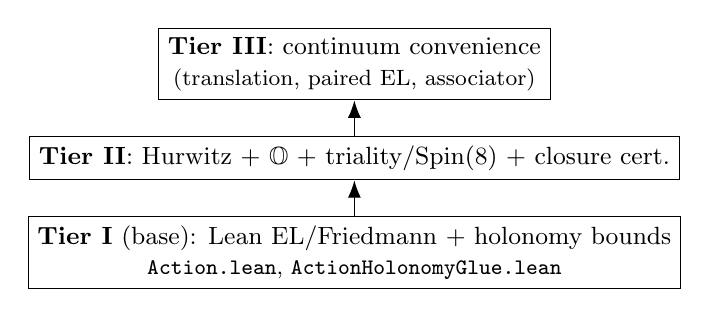
\begin{tikzpicture}[font=\small]
\node[draw,minimum width=6.8cm,align=center] (T1) {\textbf{Tier I} (base): Lean EL/Friedmann + holonomy bounds\\\footnotesize \texttt{Action.lean}, \texttt{ActionHolonomyGlue.lean}};
\node[draw,minimum width=5.2cm,align=center,above=0.45cm of T1] (T2) {\textbf{Tier II}: Hurwitz + \(\mathbb{O}\) + triality/\(\mathrm{Spin}(8)\) + closure cert.};
\node[draw,minimum width=3.6cm,align=center,above=0.45cm of T2] (T3) {\textbf{Tier III}: continuum convenience\\\footnotesize (translation, paired EL, associator)};
\draw[-{Latex[length=2.2mm]}] (T1) -- (T2);
\draw[-{Latex[length=2.2mm]}] (T2) -- (T3);
\end{tikzpicture}
\caption{Tiered uniqueness pyramid: formal theorems at the base, classical rigidity in the middle, and a continuum-convenience translation layer at the top. The discrete tier is the ontological core; the top layer is optional interoperability with standard notation. Cosmology-facing consequences of Tier~I (Friedmann constraint, \(G_{\mathrm{eff}}\), lapse dragging) are summarized in Remark~\ref{rem:lapse-lambda} and Table~\ref{tab:Geff-numerics}.}
\label{fig:pyramid}
\end{figure}

\section{Quantum scaffold and forward compatibility}
\label{sec:quantum}

\path{Hqiv/QuantumMechanics/Schrodinger.lean} defines \path{eulerLagrange_eq_Schrodinger} and proves \path{actionExtensionYieldsSchrodinger}: the extended-action EL predicate is definitionally the Schr\"odinger scaffold with the HQIV Hamiltonian template. Placeholder Laplacians remain; when Tier~III supplies optional continuum measure wrappers for comparison workflows, this module is the natural place to assert square-integrability and variational well-posedness compatible with those wrappers, including BRST or BV upgrades if the associator enters as a constraint closing ghost sectors.

\section{Outlook and roadmap for Tier III}
\label{sec:outlook}

\subsection{Minimal additional Lean scaffolds}

\begin{itemize}
\item \path{LatticeContinuumActionCoincidence}: hypothesis interface matching discrete sums to continuum integrals.
\item Controlled \emph{field} bridge lemmas \(\mathcal{R}\rightsquigarrow A\) (or \(\Delta\rightsquigarrow A\)) with explicit error terms, building on \path{ManifoldLagrangianScaffold}.
\item Discrete measure or boundary term slot for the octonionic associator, and quaternionic/sedenionic obstruction lemmas stated as \texttt{false} targets under the same ansatz.
\item Wiring \path{coordsGradientComponents} fully through both \path{EL_O_general_coordsField} and \path{emergentMaxwellInhomogeneous_O_coordsField} to close the Action \(\leftrightarrow\) ModifiedMaxwell loop.
\end{itemize}

\subsection{Milestone ordering (suggested)}

\begin{enumerate}
\item Close the Action \(\leftrightarrow\) ModifiedMaxwell gradient identification on charts (\path{ContinuumOmaxwellClosure}).
\item Promote \path{LatticeContinuumActionCoincidence} from a hypothesis structure to a theorem template with explicit rate bounds.
\item Build a functor \(\mathcal{R}\rightsquigarrow A\) on a restricted class of asymptotically HQIV configurations (partial maps first, estimates second).
\item Add non-abelian holonomy lemmas mirroring \path{L_O_kinetic_two_sided_cyclic_wilson_sq} for matrix transports in \path{DiscretePlaquetteHolonomy}.
\item Promote the weak/Higgs scaffold (\path{WeakHiggsFromOMaxwellScaffold}) from reduction-level theorems to a full EL package for weak channels and scalar sector.
\item Encode associator weights in a discrete path measure; prove quaternionic obstruction lemmas.
\item Revisit \path{Schrodinger.lean} once measure is fixed, upgrading placeholders to \path{deriv} along certified charts.
\end{enumerate}

\subsection{Dependency sketch (text)}

\[
\begin{aligned}
&\text{Growth }(\rho,K,\Omega,\mathcal{R}) &&\longrightarrow &&\alpha,\ \phi\text{-ladder} &&\text{(\path{OctonionicLightCone}, \path{AuxiliaryField})}\\
&\quad\Downarrow && &&\quad\Downarrow \\
&\Delta,\ G_2\text{ seed} &&\longrightarrow &&\mathfrak{so}(8)\text{ closure} &&\text{(\cite{hqiv-so8-paper})}\\
&\quad && &&\quad\Downarrow \\
& && &&\text{Action } \mathcal{S}_{\mathrm{tot}}
&&\text{(\path{Action.lean})}\\
&\quad && &&\quad\Downarrow \\
& && &&\text{Holonomy/Wilson packaging}
&&\text{(\path{ActionHolonomyGlue.lean})}\\
&\quad && &&\quad\Downarrow \\
& && &&\text{Tier III: continuum + measure}
&&\text{(future work).}
\end{aligned}
\]

\subsection{Thermodynamic root and lattice gauge vocabulary}

Jacobson's thermodynamic state relation for spacetime \cite{jacobson1995} is the standard conceptual ancestor of ``Einstein equation of state'' arguments; Brodie's horizon package \cite{brodie2026} is the imported normalization route for \(\alpha=3/5\) in the HQIV growth papers and feeds the same imprint into \(\mathcal{L}_\phi\) and \(G_{\mathrm{eff}}\) here. Separately, Wilson's lattice link variables \cite{wilson1974} and the textbook discrete gauge theory framework \cite{creutz1983} supply the vocabulary for reading Lemma~\ref{lem:wilson-bounds} as a small-flux plaquette inequality: the HQIV glue lemmas are not a new lattice gauge theory, but they position the O--Maxwell kinetic where Wilson-type estimates can be imported when Tier~III tightens scalings.

\appendix

\section{Lean identifier index (selected)}
\label{app:lean-index}

Table~\ref{tab:lean-index} collects identifiers used repeatedly in this manuscript; it is a reader map, not an exhaustive dependency graph (see \cite{hqiv-lean}).

\begin{table}[ht]
\caption{Selected Lean identifiers for the variational layer.}
\label{tab:lean-index}
\centering
\footnotesize
\begin{tabular}{@{}p{4.6cm}p{8.8cm}@{}}
\hline
Identifier & Role \\
\hline
\path{F_from_A} & Discrete field strength \(A^a{}_\nu-A^a{}_\mu\). \\
\path{L_O_kinetic}, \path{L_O_source_general}, \path{L_O_phi_coupling} & Kinetic, source, \(\phi\) terms. \\
\path{L_O_Maxwell_general}, \path{action_O_Maxwell_general} & Full O--Maxwell density / cell action. \\
\path{EL_O_general}, \path{action_O_Maxwell_EL_eq_emergent_general} & EL covector; equality to divergence form. \\
\path{action_O_Maxwell_general_add_J} & Nonlinear superposition correction for shared kinetic/\(\phi\) pieces. \\
\path{S_HQVM_grav}, \path{S_HQVM_grav_zero_iff_Friedmann} & Gravitational constraint scalar; Friedmann iff zero. \\
\path{action_total_general}, \path{action_total_general_add_J} & Total cell; corrected sum of two currents. \\
\path{sum_F_cyclicIndex_eq_zero}, \path{discreteSquareHolonomy_F_cyclic_eq_one} & Discrete Stokes; trivial cyclic holonomy. \\
\path{L_O_kinetic_two_sided_cyclic_wilson_sq} & Bounds kinetic by cyclic Wilson squares. \\
\path{weakF}, \path{L_weak_kinetic}, \path{higgsPotential}, \path{lockinVev} & Weak/Higgs Tier-III scaffold objects on the same discrete index spine. \\
\path{action_O_weak_higgs_reduces_exactly_to_action_O_Maxwell} & Exact reduction of extension action to proved abelian action when extension slots are zeroed. \\
\path{weakHiggs_triality_tilt_average_eq_one} & Triality CP-tilt average \(=1\) in the weak/Higgs scaffold channel. \\
\path{phi_of_shell}, \path{shell_shape_in_terms_of_phi} & Auxiliary field ladder tied to temperature shells. \\
\path{G_eff_eq}, \path{three_minus_gamma_eq} & Varying \(G\); Friedmann prefactor \((3-\gamma)\). \\
\path{HQVM_lapse}, \path{G0_eq}, \path{same_phi_in_O_Maxwell_and_HQVM} & ADM lapse \(N=1+\Phi+\phi t/c\); natural-unit \(G_0\); shared \(\phi\) for lapse/time-angle and auxiliary ladder (\emph{lapse dragging}; Remark~\ref{rem:lapse-lambda}, Table~\ref{tab:Geff-numerics}). \\
\hline
\end{tabular}
\end{table}

\section{Cross-sector compatibility (\texorpdfstring{\texttt{GRFromMaxwell.lean}}{GRFromMaxwell.lean})}
\label{app:compat}

Remark~\ref{rem:lapse-lambda} gives the expository name \emph{lapse dragging} for the morphism packaged below. The variational story is intentionally not isolated from the metric sector: \path{Hqiv/Physics/GRFromMaxwell.lean} packages a sequence of equalities asserting that the same horizon fields drive O--Maxwell and HQVM-GR bookkeeping in the homogeneous limit. Representative lemmas include \path{same_phi_in_O_Maxwell_and_HQVM} (lapse/time-angle uses the same \(\phi\) as the auxiliary ladder), \path{same_alpha_in_O_Maxwell_and_HQVM} (the lattice imprint matches the exponent in \(G_{\mathrm{eff}}(\phi)=\phi^{\alpha}\)), and \path{O_Maxwell_compatible_with_HQVM_GR_homogeneous} (Friedmann as the explicit \((13/5)\) rational form when \(\phi\ge 0\)). These files are the correct place to cite when a referee asks whether \(\mathcal{L}_\phi\) ``knows'' about cosmology: it is the same \(\alpha\) and \(\phi\) pipeline, not a second independent tuning knob.

\section*{Acknowledgments}
AI-assisted drafting and repository tooling were used during manuscript preparation. Formal claims refer to the HQIV-LEAN library; the author reviewed hypothesis lists in the cited Lean modules.

\begin{thebibliography}{99}

\bibitem{hqiv-so8-paper}
S. Ettinger Jr, \emph{From Local Rapidity Fiber to Spin(8): The Primitive Rapidity Observable and 28-Dimensional Closure}, HQIV-LEAN repository, \path{papers/hqiv_rapidity_manifold_so8_closure.tex}, 2026.

\bibitem{hqiv-3d-growth-paper}
S. Ettinger Jr, \emph{Three-Dimensional Causal Growth and the Octonionic Gauge Sector: Rigidity, Packaging, and Conditional Forcing}, HQIV-LEAN repository, \path{papers/hqiv_3d_causal_growth_octonionic_gauge.tex}, 2026.

\bibitem{hqiv-lean}
HQIV-LEAN repository, \url{https://github.com/disregardfiat/hqiv-lean}, 2026.

\bibitem{wilson1974}
K. G. Wilson, \emph{Confinement of Quarks}, Phys. Rev. D \textbf{10} (1974), 2445--2459.

\bibitem{jacobson1995}
T. Jacobson, \emph{Thermodynamics of Spacetime: The Einstein Equation of State}, Phys. Rev. Lett. \textbf{75} (1995), 1260--1263.

\bibitem{creutz1983}
M. Creutz, \emph{Quarks, Gluons and Lattices}, Cambridge University Press, 1983. See esp.\ Ch.~7 (\emph{Lattice gauge theory}: link variables, plaquette action, Wilson loops).

\bibitem{baez2002}
J. C. Baez, \emph{The Octonions}, Bull. Amer. Math. Soc. 39 (2002), no.~2, 145--205.

\bibitem{springer2000}
T. A. Springer and F. D. Veldkamp, \emph{Octonions, Jordan Algebras and Exceptional Groups}, Springer, 2000.

\bibitem{brodie2026}
K. Brodie, \emph{Derivation of Quantised Inertia from Jacobson Thermodynamics}, Zenodo (2026), doi:\,\url{https://doi.org/10.5281/zenodo.18706746}.

\end{thebibliography}

\end{document}
